\documentclass{llncs}
\usepackage{epsfig,url,graphics,code}
%\usepackage{xspace,amsmath,math-cmds,
%            math-envs,inference-rules,times,proof,
%            verbatim,alltt,multirow,multicol,url}

% correct bad hyphenation here
\input{definitions}

\begin{document}
%
% paper title
% can use linebreaks \\ within to get better formatting as desired
\title{{\sc LearnPADS}$^{++}$ \\ Incremental Inference of Ad Hoc Data Formats}
\author{Kenny Q. Zhu\inst{1} \and Kathleen Fisher\inst{2} \and 
David Walker\inst{3}} 
\institute{Shanghai Jiao Tong University \and Tufts University 
\and Princeton University}

% make the title area
\maketitle

%\begin{abstract}
%  In the age of information explosion, search engines have been an
%  essential tool in people's daily life and query suggestion is one
%  of most useful feature for a standard search engine. However, because
%  most of search engines are keyword-based, many fantastic features would
%  fail when facing concept-based queries, so does query suggestion. In this
%  paper, we propose a framework so that search engines can give acceptable
%  suggestions when facing concept-based queries.
%\end{abstract}

\begin{abstract}
  A class of search queries which contain abstract concepts are studied in
this paper. These queries cannot be correctly interpreted by traditional keyword-based search engines.
  This paper presents a simple framework that detects and instantiates the
abstract concepts by their concrete entities or meanings to produce alternate
queries that yield better search results.
\footnote{Kenny Q. Zhu (corresponding author) is partially
supported by NSFC grants 61100050 and 61033002.}
\end{abstract}

% creates the second title. It will be ignored for other modes.
%\IEEEpeerreviewmaketitle

\section{Introduction}

Protein$-$protein interactions (PPIs) are of central importance for the majority of biological functions, such as signal transduction, metabolic pathways, molecular dynamics, and protein networks\cite{Hoffmann.Krallinger.ea:2005}, for they serve as the most fundamental building blocks of the entire interacademic systems of any organisms. Collecting data on pairwise interaction relationships is essential for multiple purpose, including identification of modules with certain functionality\cite{Spirin.Mirny.03}, mapping diseases to dominated genes\cite{Ideker.Sharan.08}, and after all, understanding wholistic metabolic/genetic networks from a system biology perspective.

A lot of databases have been built to store protein and genetic interactions from major model organism species and are available in various standardized formats, such as MINT\cite{Zanzoni.Montecchi-Palazzi.ea:2002}, BIND\cite{Bader.ea:2003}, BIOGRID\cite{DBLP:journals/nar/StarkBRBBT06}, etc. Among those mainstream databases, the data largely rely on voluntary reports by scientists or researchers, besides, comprehensive curation efforts become indispensable for the sake of accuracy. However, the amount of biology-related literatures with respect to protein interactions grows explosively and thus make it either impossible or impractical to manually detect PPI information anymore.

Considering huge amount of PPI information with great wealth hidden in published papers, in recent years, numerous mining techniques have been proposed that aim to extract PPI information automatically from free text, especially machine learning, information retrieval, and natural language processing\cite{DBLP:journals/bib/WinnenburgWPDS08}.These approaches can be roughly categorized into three classes: co$-$occurrence, rule$-$based, and machine learning. 

Co$-$occurrence is the approach with most simplicity and naivete. Just as its name implies, this method intends to find out pairs of proteins that co-occur in the same context. The scope of "same context" ranges from phrase, sentence, paragraph to whole abstract, even document. The underlying assumption is that whenever two proteins are mentioned together by authors, chances are high that there is some kind of relationship between them. However, however, in-context closeness even semantic relation does not necessarily represent actual biological interaction. As a consequence, a large fraction of candidate pairs are mismatched inevitably, causing a high recall but low precision.

The second approach is rule-based extraction, in other words, pattern matching. There are many types of rules, most of them concern natural language processing (NLP). One way is to specify hand-crafted regular expressions before hand, which mostly lean on language usage preference. Besides, by using full or partial (shallow) parsing strategies, more information would be acquired, such as part-of-speech taggers, local dependencies between syntactic components, context-free grammar\cite{DBLP:journals/bioinformatics/TemkinG03}, and full sentence structure. Compared to co$-$occurrence, rule-based approach enjoy better precision but much lower recall. In addition, since the rules are usually derived from training data, that is to say, the improper choice of training data would be significantly lethal, therefore quality of extraction is invariably instable and may not applicable to other data.

The third and most commonly used approach use machine learning techniques, in this case, the task to extract protein$-$protein interactions turns out to be a binary classification problem. Each protein pairs are represented along with a set of features, which is associated with their context, then a well$-$defined classifier gives the answer whether the candidate protein pairs is classified to be qualified PPI. (TO BE FURTHER FILLED!!!)

In this paper, we introduce a general bootstrapping framework for Protein$-$protein interaction extraction from natural text.Our method differs from most of the previous works in three aspects:

(1)The extraction process is driven by only tiny fraction of training data, which are regarded as seed data. In each round, it would derive reliable patterns automatically from seed data, then extract more positive PPI pairs consequently, what's more, the seed data would be augmented by the newly extracted results with high confidence.

(2)multiple graph kernel. 

(3)various evaluation.





%%%%% ijcai19.tex



% These are the instructions for authors for IJCAI-19.

\documentclass{article}
\pdfpagewidth=8.5in
\pdfpageheight=11in
% The file ijcai19.sty is NOT the same than previous years'


% Use the postscript times font!
\usepackage{times}
\usepackage{soul}
\usepackage{url}
% \usepackage[colorlinks,
% linkcolor=black,
% anchorcolor=black,
% citecolor=black]{hyperref}
%\usepackage[hidelinks]{hyperref}
\usepackage[utf8]{inputenc}
\usepackage[small]{caption}
\usepackage{graphicx}
\usepackage{color}
\usepackage{xcolor}
\usepackage{amsmath}
\usepackage{booktabs}
\usepackage{algorithm}
% \usepackage{algorithmic}
\usepackage[noend]{algpseudocode}

\urlstyle{same}
\newcommand{\figref}[1]{Figure \ref{#1}}
\newcommand{\eqnref}[1]{Eq. \ref{#1}}
\newcommand{\tabref}[1]{Table \ref{#1}}
\newcommand{\secref}[1]{Section \ref{#1}}
\newcommand{\algoref}[1]{Algorithm \ref{#1}}
\renewcommand\appendix{\setcounter{secnumdepth}{-2}}
\newcommand{\KZ}[1]{\textcolor{blue}{Kenny: #1}}
\newcommand{\shanshan}[1]{\textcolor{blue}{ #1}}
\newcommand{\ssemp}[1]{\textcolor{red}{ #1}}
\newcommand{\scite}[1]{\citeauthor{#1}~\shortcite{#1}}

\usepackage{verbatim}
\usepackage{stfloats}
\usepackage{graphicx,amssymb,amstext,amsmath}



\begin{document}

Review1:

Comments to Authors.

I found the paper to be rather interesting but limited in its scope of what constitutes knowledge representation (and commonsense knowledge) per se. The paper limits KR to the identification of features of interest and additional information that may be gleaned from a repository such as ConceptNet. This is certainly a view of KR, but is decidedly a machine learning centric one. It would be of interest to examine works done by Lierler, Inclezan, and Gelfond regarding the application of Action Languages and logic-based KR approaches for the purpose of textual understanding as well. This perspective also limits the discussion under the related works section when the authors mention that commonsense knowledge has been shown to be effective for many inference tasks.

From a machine learning perspective though I found the paper and its approach to be of interest and the criticism of the traditional approach towards solving the "SCT story ending predicting task" sound. The proposed remedy was also of interest.

Review2:

Comments to Authors.

This paper proposes a way to use an existing structured resource such as ConceptNet to aid story modeling, approached through completion or identifying the sentiment with which a story ended. The paper extracts concepts (a graph structure) from the provided story and uses the concepts in two ways: first by obtaining dense representations of them, and second by using the concepts to help "simplify" the text of the story; this simplified text is then embedded. These two embeddings are combined into an RNN, whose final hidden representation is used to perform the classification.

The main strength of this method is that, at its core, it is a relatively simple idea that nevertheless achieves decent performance. However, this paper needs substantial editing, additional explanation of the ideas and results, and exploration of the model itself. The following lists areas for improvement:

Technical contribution:

The paper uses negative sampling to train the model, yet erroneously refers to this as a semi-supervised method.

\shanshan{Thank you for pointing out this mistake on our part. Our approach is indeed supervised classification using negative sampling. We will modify the wordings in the revised version and also adjust the headers in Table 4 to "Unsupervised" and "Supervised" respectively.}

 \ssemp{This paper relies on ConceptNet and Numberbatch; it's unclear what exactly in that representation is helping performance. Put another way, is the idea of concept extraction and text simplification a generalizable method (and ConceptNet provided the means), or is there something specific to ConceptNet and Numberbatch?}
 
 \shanshan{The framework proposed in this paper, that is, text simplification plus structured commonsense knowledge is general and can be applied to other commonsense knowledge graph than ConceptNet. We used ConceptNet here due to its comprehensive coverage and relatively high quality. Our contribution here is this framework that makes good use of the knowledge in ConceptNet. If there were a similarly structured but better knowledge source, we are certain it could be plugged into the framework and yield better results. For example, when we use half of ConceptNet in a separate experiment, the results are.... }
		
Clarity:

	\ssemp{The paper needs to spend much more time describing the underlying resources used (ConceptNet and NumberBatch), the algorithm used (what does "word length" for a concept mean? see Sect 2.1), and the impact of their modeling decisions.
	The paper needs thorough proof-reading: there are systematic grammatical errors (e.g., the omission of determiners) that make the paper difficult to read.} 
	\shanshan{We will describe ConceptNet and NumberBatch more clearly in the revised version and proofread the whole paper carefully. 
``word length'' means the number of words in a concept. We will rephrase this term to ``length of a concept''.}

Scholarship:

\ssemp{The paper mischaracterizes at least one work: SemLM (Peng \& Roth, 2016) relies on the output of automated frame and entity tools.}	

\shanshan{Actually in Sec 4, para 2, we were discussing a number of end-to-end techniques for SCT using "manually chosen features". 
SeqMANN is one such technique making use of a feature called SemLM, which is extracted from external resources. So what we are categorizing is
really SeqMANN, and not SemLM. We will rephrase the sentence to make it clearer in the revision.}  

This paper covers story cloze tasks well, but does not sufficiently consider larger implications/connections of the method. For example, other methods of event simplification (Orr et al., 2014 AAAI; Ferraro \& Van Durme 2016, AAAI; Picchota \& Mooney 2016, AAAI).

\shanshan{As the title of the paper suggests, we are limiting our research to representing stories using commonsense knowledge. Orr, Ferraro, Picchota ,
}

Review3:

Comments to Authors.

The paper proposes a model that leverages common sense knowledge for story end prediction. In particular, the facts from ConceptNet are used to simplify the story by extracting a sequence of ConceptNet concepts from the sentence and then, the latent relationship among the key ideas in the story is modeled and finally, a GRU based classifier is used to predicts the correct ending. The model is evaluated on ROC Story Cloze Test data set.
The paper is poorly written and not well-motivated. Also, the technical novelty of the paper is very limited. Here are some concerns/issues regarding the work as listed below–

1.    In Sec 1., authors say- "Predicting “what happens next” in narrative stories is an important but challenging task called commonsense reasoning in artificial intelligence."  – The statement provides a narrow definition of commonsense reasoning problems that exits in AI and is not quite appropriate.

	\shanshan{Our abstract says ``Predicting ending for narrative stories is a grand challenge for machine commonsense reasoning,'' and this is what we really wanted to say.  We will fix this erroneous setence in the introduction in revised version.}
	
2.    In Sec1,  ``Instead, we propose to define the SCT story ending predicting task as a semi-supervised learning problem" – Why you consider the task as semi-supervised learning? More elaboration is required to clearly define the task and explain the notion of  ``semi-supervised learning".

	\shanshan{Please refer to R2...}

3.   The proposed approach is dependent on simplifying the sentence representation by extracting key concepts and mapping them using ConceptNet…What happens if none of the concept in the given sentence or end sentence is found in ConceptNet? How the model deals with Out of Vocabulary (OOV) concepts?…Any empirical analysis on how it affect performance when there is more OOV concepts in the story.

	\shanshan{Our preliminary study shows that only 0.034\% of the sentences from the ROCStories data do not contain any ConceptNet concepts. 
Furthermore, fewer than 0.017\% of the ending sentences of a story contain no concept at all. Therefore we consider the OOV problem to be statistically 
insignificant and choose to ignore it. We add the above discussion to the Sec. 3.} 

4.  In Sec 3,..  ``Then we present a preliminary analysis on the ROCStory dataset to invalidate previous approaches…" – Do you mean previous approaches are all invalid for the task? ..why?

	\shanshan{As we pointed out in Sec 3.2, the previous methods are not invalid, but because they were all trained on the validation set which has information leak, their evaluation results are therefore invalid.}

5.  In Sec 3.2,.. ``The fact that humans score substantially worse than some of the `top' algorithms indicates that these algorithms are not using “commonsense” but rather the patterns leaked in the training data." --- ISCK model combines information like sentiment, commonsense and narrative sequence representation for story end prediction. Why ISCK model is not included in Table 3? Based on the explanation of information leak, have you considered comparing ISCK without sentiment information? From the ablation study conducted by Chen et.al. 2018, it seems like ISCK is still a strong model considering only commonsense knowledge version on ROC stories corpus.

\shanshan{In Table 3, we show the result for models trained only with story endings. However, ISCK requires sentiment and commonsense features which cannot be trained using the last sentence of a story alone. Thus it is not included in Table 3. Table 3 is there to illustrate the information leak problem and is not our main result. We did compare with ISCK in Table 4, which is our main results. We didn't compare with ISCK without sentiment because according to Chen 2018. that setup is worse than the ISCK model itself.} 

6. The results of FTML on SCT dataset in the paper differs substantially from that Radford et. al. -- any reason? Why results on ROCStories Test set have not been reported?

	\shanshan{What we report in this paper are indeed results on the SCT test set, same as in previous work on the task. The reason for the different results of FTML was explained in Sec 3, mainly due to the use of different training data.} 
	
7. In sec 3.3., ``In fact we logged 5\% improvement over RNN-BC which was the previous state-of-the-art." – which model is RNN-BC ..I can not see any information on Table 4 and sec 3.1. 

\shanshan{RNN-BC should be SKBC. This is a typo.}

Review4:

Comments to Authors.

This paper proposes and implements a methodology for determining
the end of a short story, by selecting one among two possible
endings. The process (seems to) identify concepts in the sentence
that also appear in ConceptNet, identify relations in ConceptNet
that relate those concepts, and then use learning over a training
set of data whose negative labels are created automatically to
learn how to predict the correct ending in a given testing set.

The problem seems interesting, in that it has potential to be
extended to question answering in stories, which itself is a an
important problem for commonsense reasoning. To my understanding,
the solution is also potentially interesting in that it combines
symbolically-represented knowledge from ConceptNet with deep
learning techniques to create a predictive model for the task.

\ssemp{I found it very difficult to follow the paper. It presents the
technical parts of the methodology at a very high level, making it
hard to appreciate how various things have been implemented. A
running example and many more technical details would seem
necessary, especially since the paper has extra space that it could
use. As it stands, the paper cannot be said to be self-contained.}

Also, there is a lot of work in the literature that makes the point
that the use of symbolically-represented knowledge is a central
component in both human and computational story understanding
(e.g., work by Michael and colleagues on ``Story Understanding...
Calculemus!" and ``Knowledge Activation in Story Comprehension"). In
particular, the literature seems to suggest that causal knowledge
(which does exist in ConceptNet, but might be only a small
fraction) is the key form of knowledge used in story understanding.
The authors might want to consult this literature and see how to
adapt their approach to get even better results, or to offer
evidence for or against the suggested role of causal knowledge.

The paper must be checked for the proper use of English.

A minor point: Claiming that the words not highlighted in Figure 1
are not important in the understanding of stories is simplistic.
Pronouns, for example, sometimes play a key role in story
understanding, and cannot simply be ignored. You may want to
rephrase the claim to say that you simply ignored those words.

\shanshan{Thank you for the suggestions. We will carefully proofread the 
paper, improve English and clarify important details in the revised version.
In this paper, our main contribution is in fact the discovery 
that commonsense concepts plays an important role in understanding 
the logic of stories. Hence we choose to ignore other parts of 
the sentences such as pronouns and person names.}
		
\end{document}


\section{Technical Specification}
\label{sec:tech}

\begin{figure}[h]
\begin{center}
\epsfig{file=archi.eps,width=0.85\columnwidth}
\caption{PredicTV System Architecture}
\shrink
\label{fig:archi}
\end{center}
\end{figure}

Figure \ref{fig:archi} illustrates the system architecture.
The core recommendation engine consists of two modules:
the offline web information extraction module and the online
recommendation module. The first module collects in advance weekly TV schedule,
identifies program titles and show times, and then extracts relevant
information about programs from web. 
The second module maintains user viewing model
dynamically and by comparing the similarity between the 
current user model and programs, 
recommends the most relevant programs to the user in real time.
We next present these two modules in greater details.

%Communication module receives users' channel switching requests,
%transfers them to Recommendation module, and outputs
%recommendations to the user. Database module stores all the program
%models and dynamically changing user viewing models. We next focus on
%the other key components: information extraction module and
%recommendation module.
%
%The Information Extraction module has two tasks. One is to crawl HTML pages  
%about TV programs from the internet, another is to extract 
%important attribute-value pairs from the pages. 
%We use Baidu and Google for the first task. 
%%For a program
%%that we want to collect its information, we form an URL based on Baidu
%%and Google's rules. Then we send HTTP requests to both these two sites
%%and get replies. Baidu and Google will reply the URLs of websites most fit
%%the key word we provide, so we send HTTP requests again and get HTML files
%%we need. Though Baidu and Google help us to search the websites most
%%related to our key words, there will still be some noise in the HTML files,
%%so we define some patterns to match information we need.
%
%Recommendation module is the core of our system. It uses users' viewing
%behaviour information as the
%input of its analysis process then replies recommendation results to users
%via Communication module. Since in mainland China, we don't have standard
%and detailed TV program information available, we have to obtain such
%information ourself. That's why Information Extraction module is involved
%in our system. It grabs HTML files from the internet, filters unnecessary
%parts, then passes them to Recommedation module. 

\subsection{Program and Viewer Model}
Before discussing the details of the two modules, we first introduce the
structure of our program and viewer model. A program model is basically a list
of attribute-value pairs. Attribute is the property of 
a program such as director, 
cast of a movie, or host of a talk show.
For certain attribute like cast of a movie, 
the value can be a set of names rather than
a single value.
In order to extract such properties or attribute values, 
we employ a statistical method.
First, we gather the list of programs, and then use 
search engine to find related pages of these programs. 
In the pages returned, we use simple but strict patterns to
match key-value pairs then choose keys which appeared more frequently 
to form an attribute list. 

A viewer model is the accumulation of program models, so the structure
is the same with program model. 
What's different is that in program model, each attribute-value
pair contains a set of values, whereas in viewer model, each value is also
is associated with a weight, which represents how important that 
value is for the owner of the model.

\subsection{Web Information Extraction}
The module first run a crawler to download TV
schedules for the coming week. As long as schedules are ready, 
before we use search engine to find out related pages for programs, 
we need to do some preprocessing on the program
name, because program names in the TV schedule may contain 
noises like type, subtitle and episode number, which affect the results
returned from search engine. After preprocessing, 
the modified program names are put on search engines like Google and Baidu. 
Ideally we will get many related
pages containing the information we need. 
As discussed in previous section, we automatically
form an attribute list for program model. 
For each attribute, we use a simple pattern to match
the context of that attribute and extract values for that attribute.

\subsection{Model Update and Recommendation}
When a viewer turns on TV, she may switch between different channels.
We capture her actions and try to predict her likes and dislikes. 
From the viewing history, we can collect the duration the viewer
views each program. We assume that the longer viewer views one program, 
the more she likes that program. 
We use this criteria to update viewer model. 
When the viewer switch to a new channel, 
a viewing record containing the old channel id, 
timestamp and duration viewer stays on that
channel is sent to server. According to channel id and timestamp, 
we find out what program viewer was previously 
watching and get the program model for viewer model updating. 
We merge program model into viewer model. 
The duration the user has spent on a program is translated into
the weight for each value in viewer model. 
All values in program model will be added to viewer model. 
If viewer model already contains that value, the weight of value will be
increased, otherwise that value is directly added to viewer model. 
We have a restriction on the size of value
set in each attribute. If the set is full, 
we remove value with the lowest weight. 

In the recommendation step, we first get a list of candidate programs to
be recommended. These are typically programs shown right now or in the near 
future. For each program in the list, we calculate the similarity 
between that program model and viewer model using Equation (\ref{eq-sim}),
and we return the top 3 programs as recommendation result. 

\begin{equation}
P_u(p) = \sum_{i=1}^nw_i\delta(v_{u_i},v_{p_i})
\label{eq-sim}
\end{equation}

$\delta(v_{u_i}, v_{p_i})$ is used to calculate the similarity between value of users and value of programs.
For each attribute in the attribute-value list, 
taking into account the different types of attributes, we design three
different implementations of function $\delta(v_{u, i}, v_{p_i})$.

For title, its value is normally a single chinese string. 
Comparing the whole string is not good enough,
therefore we use a segmentation tool to split the whole string 
into several phrases to form a set, and use Jaccord similarity here.

For time, since its value is a range, we can calculate the intersection and union of two time
range. Then divide the length of intersection by the length of union and use the ratio as the similarity.

For other attributes, the value of the attribute is also a set, so we also use Jaccord similarity, but we make some change this
time. When calculating both the intersection and union, for every value in the intersection or union, instead of
adding 1 to the size of intersection or union, we add the weight of that value. So the size here is a weighted size.

In our equation, each attribute similarity has a weight parameter $w_i$. 
Our concern is that
for different users, the effect of one attribute which influences user's choice is different. $w_i$ is
used to define the importance of one attribute to users. For each attribute, 
$w_i$ is the max value weight divided by
the sum of value weight in that attribute.


\section{Implementation}
\label{sec:implement}

In this section we first attempt to experimentally 
determine the value for three key 
paramaters in our framework and then describe a baseline system for comparison
with our framework.
\cut{We also discuss the possibility to incorporate other data sources in building the co-occurrence matrix.}
%\subsection{Matrix Storage}
%As discussed in \secref{sec:enrich}, the co-occurrence matrix is very sparse
%because many pairs of Wikipedia concepts will not appear together in
%the Wikipedia corpus. Therefore instead of using a two-dimension array, we
%use a hash table to store the co-occurrence information. For each pair, we
%combine the IDs of the two Wikipedia concepts to form a key,
%and use the co-occurrence frequency as the value.

\subsection{Parameter Settings}
\label{sec:config}
The key parameters in our framework include $\tau$ which determines whether
to disambiguate a given term in our matrix enrichment process,
$W_c$, the co-occurrence window size in the iterations, and $W_s$, 
the sliding window size for wikifying new documents. 
%This subsection describes how these parameters
%are experimentally determined.

For threshold $\tau$, we randomly pick 100 paragraphs from Wikipedia corpus. We use function \emph{UpdateArticles} in
Algorithm \ref{enrich} to add links to these paragraphs using the matrixes
generated by the enrichment process on different thresholds.
We also manually add links to these 100 paragraphs, as ground truth labels.
We compare the different linking results with the ground truth then calculate the
precision and recall, which is shown in Table \ref{tab:theshold}.

\begin{table}[th]
\centering
\begin{tabular}{|c|c|c||c|c|c|}
\hline
$\tau$ & Precision & Recall & $\tau$ & Precision & Recall \\
\hline \hline
0.1 & 87.50\% & 40.94\% & \bf{0.5} & \bf{90.16\%} & 64.50\% \\
0.2 & 90.04\% & 63.66\% & 0.75 & 89.62\% & 66.01\% \\
0.25 & 89.29\% & 63.74\% & 0.875 & 88.89\% & 68.57\% \\
\hline
\end{tabular}
\caption{Result on Different Thresholds (with co-occurrence window $W_c$ = 15)}
\label{tab:theshold}
\end{table}
\cut{
\begin{table}[th]
\centering
\begin{tabular}{*{3}{|c}|}
\hline
Threshold & Precision & Recall \\
\hline \hline
0.1 & 87.50\% & 40.94\% \\
0.2 & 90.04\% & 63.66\% \\
0.25 & 89.29\% & 63.74\% \\
\bf{0.5} & \bf{90.16\%} & 64.50\% \\
0.75 & 89.62\% & 66.01\% \\
0.875 & 88.89\% & 68.57\% \\
\hline
\end{tabular}
\caption{Result on Different Thresholds (with co-occurrence window $W_c$ = 15)}
\label{tab:theshold}
\end{table}
}
We can see that threshold 0.5 achieves the best precision and also
reasonable recall. Since our matrix enrichment process is an
iterative process, precision in each iteration is more important, we
therefore choose 0.5 as threshold $\tau$.
%\KZ{Notice that $\tau$ is a
%parameter that affects the number of iterations at runtime.}

For $W_c$, we follow the same experiment described above,
since these two parameters are both used in the matrix generation part.
Instead of using different thresholds, we change the window size this
time. Table \ref{tab:window} shows the linking precision and recall 
using different $W_c$. 5 and 15 both achieve precision
higher than 90\%. To optimize the recall, we set $W_c = 15$.

\begin{table}[th]
\centering
\begin{tabular}{|c|c|c||c|c|c|}
\hline
$W_c$ & Precision & Recall & $W_s$ & Precision & Recall \\
\hline \hline
5 & 91.67\% & 45.20\% & 2 &84.59\%&	52.74\% \\
10 & 89.63\% & 60.84\% & 3 &84.95\%& 83.47\% \\
15 & 90.16\% & 64.50\% & 4 &85.52\%& 88.68\% \\
20 & 88.30\% & 67.05\% & 5 &85.55\%& 89.60\% \\
\hline
\end{tabular}
\caption{Result on Different $W_c$ and $W_s$ (with threshold $\tau$ = 0.5)}
\label{tab:window}
\end{table}

For $W_s$, we build another test data with 100 randomly picked paragraphs
from web and wikify them using the sliding window algorithm. The matrix used in
this experiment is generated by enriching 10,000 sample Wikipedia articles, 
with parameters $\tau= 0.5$ and $W_c=15$. Table \ref{tab:window} compares 
the results on different $W_s$ with the manually created ground truth.
Both precision and recall increase with growing $W_s$. 
When $W_s$ is larger than 5, the whole process takes too much time and 
is thus not practical. Consequently we set $W_s = 5$.

%\begin{table}[th]
%\centering
%\begin{tabular}{*{3}{|c}|}
%\hline
%$W_s$ & Precision & Recall \\
%\hline \hline
%2 &84.59\%&	48.12\% \\
%3 &84.95\%&	72.72\% \\
%4 &85.52\%&	77.10\% \\
%5 &85.55\%&	77.82\% \\
%\hline
%\end{tabular}
%\caption{Result on Different $W_s$}
%\label{tab:windows}
%\end{table}
\cut{
\subsection{Boosting of Common Terms}
One challenge we discuss in \secref{intro} is that some common and
``easier'' terms are usually less linked than popular and
``difficult'' terms.
%This biased distribution of links affects our overall iteration results.
%When these terms appear in an article, it is more likely it bears
%the most general sense.
For example, when ``Country'' appears in an article,
its sense is usually the general one, which means a region legally
identified as a distinct entity in political geography.
Less often does it mean ``Country music''.
However, in the Wikipedia corpus, the term ``Country'' is rarely linked to
its general sense because it's not ``link-worthy''.
Consequently, our iteration process is not likely to link such common terms
to their general senses, either.
Instead, common terms can be mis-linked to their special senses.

To avoid this problem, we apply the following approach to ``boost'' the most
general sense of common terms.
For each term in the original corpus, we count the number of times
it is unlinked vs. linked. We compute a ratio
\[r = \frac{f(unlinked)}{f(linked)+f(unlinkded)}
\]
between the unlinked frequency and the sum of unlinked frequency and linked frequency.
Our assumption is that, the higher this ratio is, the more
likely this term is using its general sense.
Subsequently we adapt $S_{CC}$ in
\secref{sec:enrich} to:
\[ {S_{CC}}^\prime\left(c\right)=\left\{
\begin{array}{r@{\;\;}l}
g\left(r\right)\cdot S_{CC}\left(c\right) & \mbox{if c is a general sense}\\
g\left(1-r\right)\cdot S_{CC}\left(c\right) & \mbox{if c is not a general sense}
\end{array} \right.
\]
where $r$ act as a boost factor for the general sense
when the term is a common one, $g$ is a monotonically increasing
function of $r$ that adjusts the impact of boosting.

To discover function $g$, we sample 10,000 articles from Wikipedia corpus then count the
linked frequency and unlinked frequency of each terms. We sort all the terms based
on $r$. According to our observation, only terms with extremely high $r$ are likely
to be ``easier'' terms. For example, ``year'', with $r$ equals to 0.999, is
usually used as a time unit, which is its common sense. However, ``apple'',
with $r$ equals to 0.863, is usually used in the senses of a kind of fruit
and a technology company. Thus, we fit function
$g$ shown in \figref{fig:gfun}. The intuition is to give those terms with very
high $r$ (nearly 1) a boost.

\begin{figure}[th]
\centering
\epsfig{file=figure/gfunction.eps,width=0.6\columnwidth}
\caption{Function $g$}
\label{fig:gfun}
\end{figure}
}
\subsection{Baseline System}
Besides the algorithm introduced in \secref{sec:framework},
for comparison purpose,
we also implemented a baseline system which wikifies a document by the
co-occurrence between Wikipedia concepts and plain words.
This system can be thought of as a direct port of WSD from using WordNet to
using Wikipedia, and it also uses a common bag-of-words approach.
In this baseline system, the co-occurrence vector of
each Wikipedia concept is constructed
from words and frequencies in the article of this concept itself.
With the vectors of all Wikipedia concepts,
we can wikify a document by comparing the co-occurrence vectors with
the context of each term in the document. Given a document, we parse it
into terms in the same way as our wikification framework.
Each term has a list of candidate Wikipedia concepts.
We compute the cosine similarity
between the vector of each candidate concept and the vector built from
the input document. The concept whose vector has the best similarity with
the document vector is chosen to disambiguate that
term. We compare the result of this baseline system with
our wikification framework in \secref{sec:eval}.

%\subsection{Beyond the Wikipedia Corpus}
In this paper, Wikipedia acts as a lexicon which provides all the
surface terms as well as concepts to link to for wikification.
However, even though the Wikipedia text
corpus itself is very large, it is unlikely to contain all the co-occurrence
information there is between any two concepts. Additional data sources maybe
used to provide co-occurrence evidences not seen in Wikipedia itself.
For example, suppose in the Wikipedia corpus, concepts $a$ and $b$ co-occur,
concepts $a$ and $c$ also co-occur, but there's no evidence which supports
the co-occurrence of $b$ and $c$. Now, given a new plain text document, because of the co-occurrence between $a$ and $b$ and the co-occurrence between $a$ and $c$,
we may be able to disambiguate three terms $t_a$, $t_b$ and $t_c$ to $a$, $b$,
and $c$, respectively in the document. Consequently, a new occurrence ($b$, $c$)
which was never seen in Wikipedia itself, can be discovered and added to our
co-occurrence knowledge.
%Not only Wikipedia corpus, we also consider the possibility to bring in
%other source to help us collect more co-occurrence information. Plain
%text on web is a candidate. We are interested in the word and phrase
%distribution on both Wikipedia article and plain text.

We conduct the following experiment to verify our hypothesis.
We randomly sample 10,000 web pages from a Bing snapshot and
extract plain text from them.
Then we randomly pick two groups of 10, 000 Wikipedia articles, called
Wiki-1 and Wiki-2. We compute the word distribution and the Wikipedia terms
(phrase) distributions from these three groups of text and measure the
the cosine similarity between word distributions and between
phrase distributions in Table \ref{tab:vector}.

\begin{table}[th]
\centering
\begin{tabular}{|c|c|c|}
\hline
Data Sources           &  Word Similarity &  Phrase Similarity \\
\hline \hline
Wiki-1 vs. Wiki-2 &      0.992 &       0.990 \\
Plain text vs. Wiki-1 &      0.633 &      0.765 \\
Plain text vs. Wiki-2 &      0.629 &      0.764 \\
\hline
\end{tabular}
\caption{Word and Phrase Distribution Similarity}
\label{tab:vector}
\end{table}

Table \ref{tab:vector} shows that the word and phrase distribution
between two Wikipedia sets are very similar.
Whereas both word and phrase distribution of plain text share lower
similarity with those of the two Wikipedia sets. This indicates that
data sources outside of Wikipedia do have significant differences and hence
have the potential of introducing fresh co-occurrence information into
the Wikipedia corpus.

One straightforward way of incorporating the co-occurrence data from other sources
into Wikipedia is to wikify the plain text,
calculate co-occurrence frequency between the concepts inside a window, and then
update that information into the co-occurrence matrix we obtained from
Wikipedia itself.
We use the matrix generated from 10,000 sample Wikipedia articles to wikify
10,000 other web pages. Results show that this process introduces 2,802,392
fresh pairs, which is 10.47\% of the original matrix size.

%Our iterative algorithm that enrich the co-occurrence matrix can not only
%be applied on Wikipedia articles, but also plain text, which can bring us
%more knowledge. The process is similar to what we use to wikify plain text
%document. We set a sliding window and calculate the ($S_{SW}$)s. But instead
%of finding the best sense for each term, we delete the worst sense in each
%iteration with the lowest sum of ($S_{SW}$)s.
%
%The whole process on plain text starts with an initial co-occurrence matrix,
%which can be generated by the process on Wikipedia articles. In each iteration,
%each existing sense of a term is assigned a value which is the sum of all the
%($S_{SW}$)s this sense contributes to. The sense with the lowest value is deleted.
%Once there is only one sense left for a term, or to say the sense of that term
%is fixed, we add a link to the corresponding document and update the co-occurrence
%matrix. The iterations continue until no link can be added.





\section{Experiments}
We first expound our pruning setting
and provide evidences for its ability to identify relation-specific subnetworks in PLM.
Then we experiment on several commonsense-intensive scenarios to seek 
good practices for using these subnetworks.

\subsection{Disentangling PLMs into Relation-specific Subnetworks}
\label{sec:LAMA}
\begin{table}[!h]
	\centering
	\small
	\begin{tabular}{l|cc}
		\toprule
		\textbf{Data Split} & \textbf{\# Rels} & \textbf{\# Prompts} \\
		\midrule
		Train  & 16 &  20,841\\
		Validation   & 16 &  5,955\\
		Test   & 16 &  2,978\\
		\bottomrule
	\end{tabular}
	\caption{Statistics of C-LAMA.}
	\label{table:conceptnet}
\end{table}
\noindent
\textbf{Dataset.}~~We use the ConceptNet~\citep{speer-havasi-2012-representing} subset of LAMA benchmark as supervision, denoted as C-LAMA.
C-LAMA contains commonsense facts from the English part of ConceptNet that has
single-token objects covering 16 relations. These facts are extracted from Open Mind Common Sense~(OMCS) and will be used as cloze-prompts for pruning. We construct the train/valildation/test splits with a ratio of 7:2:1. Detailed statistics is listed in \tabref{table:conceptnet}. Precision P@K is used to evaluate the prompt filling performance. For a given $\mathcal{LM}$, we save subnetworks that achieve highest micro-averaged P@1 on the validation set and report the micro-averaged P@K on the test set.
%\KZ{What confuses me a bit is that the pruning matrices are trained on C-LAMA, and then testedb-[]
%also on C-LAMA, then what makes it a weak-supervision? How do you determine the train-test split
%on C-LAMA?}


\noindent
\textbf{Models.}~~For the choices of $\mathcal{LM}$, we consider the 6-layer \textsc{DistilBERT-base}~\citep{DBLP:journals/corr/abs-1910-01108}, 12-layer \textsc{BERT-base}, 12-layer \textsc{RoBERTa-base}~\citep{DBLP:journals/corr/abs-1907-11692}. We also include the more recent 12-layer \textsc{MPNet-base}~\citep{song2020mpnet} model. All models are implemented with HuggingFace's transformers~\citep{DBLP:journals/corr/abs-1910-03771} library. 

\noindent
\textbf{Setup.}~~The prior distribution $\phi(\cdot)$ is a Gaussian $\mathcal{N}(\mu, 1)$ where $\mu$ is the mean controlling initial sparsity of pruned model~(e.g., $\mu=0$ indicates $50\%$ initial sparsity).
We set $l_t$ to be the top layer of a given model 
and choose $l_b$ from $\{3,4\}$ for \textsc{DistilBERT}, $\{6,7,8,9\}$ for \textsc{BERT}, \textsc{RoBERTa}, 
and \textsc{MPNet}. The temperature $\tau$ is fixed as $0.1$. The threshold $t$ is fixed as $0.5$. 
We use Adam~\citep{kingma2014method} with a batch size of $32$ and a linear warm-up scheduler 
with $0.1$ warm-up ratio for training the mask up to $6$ epochs. 
The learning rate is fixed as $3\times 10^{-4}$. All experiments are conducted on a GTX 1080 Ti GPU with 11G RAM.
% \KZ{Table 1 indicates
%that the sparcity of all three models under deterministic pruning is around 50\%, which is the same
%as the initial sparcity. This means nothing is done?? Also this sparcity issue seems not mentioned in the method section?
%How we do control the sparcity? Why do we need to control it? Does it have anything to do with the accuracy of
%the subnet thus obtained?} 


%\KZ{The organization of the following experiments seems a bit
%arbitrary. Maybe first give an overview of what experiments will be done next
%and their logical connection?}
\begin{figure}[t!]
	\centering
	\scalebox{1.0}{\includegraphics[width=1.0\columnwidth]{figure/both.pdf}}
	\caption{Ablation on the pruning masks~(left) and effect of initial sparsity and pruned layers~(right).} \label{fig:both}
\end{figure}
\noindent
\textbf{Factors impacting performance.}~~~To investigate how $\mu$ and $l_b$ influence the  performance, we perform a preliminary experiment by applying deterministic pruning on \textsc{BERT-base} with $l_b$ in $\{6,7,8,9\}$ and initial sparsity in $\{50\%,54\%,58\%,62\%\}$.  \figref{fig:both}~(right) shows that (i)~increasing the number of pruned layers helps distill more knowledge. (ii)~larger initial sparsity is more likely to prune away weights important to certain knowledge and cannot be recovered in the later training process. In general, we find an initial sparsity around $50\%$ yields decent performance both in probing and downstream applications. We adopt this setting in the remainder of this paper unless state otherwise.
\begin{table*}[t!]
	\centering
	\scriptsize
	\begin{tabular}{l|ccc|c|c|c}
		\toprule
		\textbf{Model} & \textbf{P@1~(\%)} & \textbf{P@2~(\%)} & \textbf{P@3~(\%)} & \textbf{Sparsity}  & $\bm{l_b-l_t}$ & \textbf{\# Param.}\\
		\midrule
		\textsc{DistilBERT} w/o pruning& 11.4 &16.6  &19.9  & 0\% & - & 66M\\
		\textsc{DistilBERT} w/ stochastic pruning & 14.8 &21.5 &26.3 & $\sim$30\% & 4-6 &66M \\
		\textsc{DistilBERT} w/ deterministic pruning & 44.1 &52.9 &57.6 & $\sim$50\% & 4-6 &56M \\
		\midrule
		\textsc{BERT} w/o pruning& 12.9 & 18.4  & 21.8 & 0\% & -  &110M\\
		\textsc{BERT} w/ stochastic pruning & 17.2 & 25.1  & 29.6  & $\sim$30\% & 7-12 & 110M\\
		\textsc{BERT} w/ deterministic pruning & 57.6 & 63.8  & 67.2  & $\sim$50\% & 7-12 & 88M\\
		\midrule
		\textsc{RoBERTa} w/o pruning& 15.4 & 21.2  & 24.6 & 0\% & - &125M  \\
		\textsc{RoBERTa} w/ stochastic pruning &16.6  &22.2   &25.8   & $\sim$30\% & 7-12 & 125M\\
		\textsc{RoBERTa} w/ deterministic pruning &38.3  &42.8   &44.6   & $\sim$50\% & 7-12 &100M \\
		\midrule
		\textsc{MPNet} w/o pruning& 14.8  &20.7   &24.0 & 0\%  & - & 110M\\
		\textsc{MPNet} w/ stochastic pruning &19.8  &27.9   &33.2  & $\sim$30\% & 7-12  & 110M\\
		\textsc{MPNet} w/ deterministic pruning &62.7  &68.7   &71.4  & $\sim$50\% & 7-12 &88M \\
		%		\midrule
		%		\textsc{BERT-base-finetuned-CoNLL03} w/o pruning&0.0  &0.0   &0.0 & 0\% & -  & 110M\\
		%		\textsc{BERT-base-finetuned-CoNLL03} w/ deterministic pruning & 27.1 & 37.7  & 43.1 & $\sim$50\% & 7-12 & 88M\\
		%		\midrule
		%		\textsc{BERT-base-finetuned-SQuAD} w/o pruning&0.0  &0.0   &0.0  & 0\% & - & 110M\\
		%		\textsc{BERT-base-finetuned-SQuAD} w/ deterministic pruning & 22.5 & 32.4  & 37.5 & $\sim$50\% & 7-12 & 88M\\
		\bottomrule
	\end{tabular}
	\caption{Relational knowledge probing results on C-LAMA. We relegate the 
		complete results to Appendix.}
	\label{table:rank}
\end{table*}

\noindent
\textbf{Disentanglement between subnetworks.}~~Properly disentangled subnetworks are expected to perform poorly on relations other than their associated ones. We verify this by instantiating the pruning mask upon \textsc{BERT-base} with a set of mismatched masks.
Specifically, we corrupt the correspondence of relation between masks and prompts by shifting the order of masks 15 times, as there are 16 relations in total. Then we calculate the micro-averaged P@K for each shift and average the results. As shown in \figref{fig:both}~(left), If we apply the mismatched masks from other relations, the P@1  score significantly drops to $4.8$, even inferior to the original model. It shows that the representation spaces for different commonsense relations modeled by these subnetworks are highly disentangled and  exhibits remarkably distinct geometry.

We also examine the non-triviality of subnetworks by initializing the masks with a Bernoulli distribution $B(0.5)$ and averaging the results from 5 different random seeds.
If we apply such random masks with sparsity comparable to learned ones, the P@1 drops drastically to $0.4$. This notable gap proves that the effective subnetworks cannot be trivially identified through random weights sampling.

\noindent
\textbf{Comparision with original models.}~~We present the full results of all models in \tabref{table:rank}. Among all models without pruning, \textsc{RoBERTa} achieves the highest P@1 score of $15.4$ while \textsc{DistilBERT} gets the lowest $11.4$. It indicates that while PLMs are shown to be helpful for downstream learning, they cannot accurately complete cloze-like prompts that require commonsense relation knowledge. This observation also coincides with previous finding~\citep{inductivemlm} that the uniform masking adopted by PLMs is biased towards extracting statistical and syntactic dependencies. 
Comparing the results for each pair of original and subnetworks, we consistently observe a surprisingly significant increase~(37.0 on average), especially for deterministically pruned ones. This large performance gap provides unique new evidence of sparse latent relational knowledge structures in PLMs, which are weakened by pretrained weights that are \textit{reserved} for more general-purpose use. 

We also observe that the deterministic pruning excels by a huge margin 
across all models, which implies that representation subspaces for relational knowledge deviate largely from the original language representation space. Another advantage of deterministic pruning in memory 
footprint is that only sets of 1-bit masks rather than 32-bits float parameters 
need to be saved for solving multiple tasks. For the above reasons, 
we focus our analysis on and use \textsf{pruned} to denote deterministically 
pruned PLMs in the rest of this paper. 
%\KZ{Why deterministic ones are so much better than stochastic ones?
%THis is a bit counter-intuitive.}
%\KZ{To show that you have successfully disentangled the network into 16 subnets, each corresponds to a relation
%in C-LAMA, maybe you should also show that a subnet for $r_i$ works not so well for relation $r_j$ where
%$i \ne j$, but works very well for $r_i$?  Later in Fig 2 (left) you showed this result. But does it come a bit too
%late? You have only showed the latter in Table 1. But of course, $r_i$ and
%$r_j$ need to be semantically distinct in the first place.}



%\KZ{What's the diff between this subsubsection and the previous one about ``to what extent we can
%disentangle? It seems that to show the extent u can disengle u need to show that
%the subnets are very different? But that's doesn't seem to be so important.
%Maybe u can consider merging these two subsubsections.}


%\begin{figure}[t]
%	\centering
%	\scalebox{1.0}{\includegraphics[width=1.0\columnwidth]{figure/vertical.png}}
%	\caption{Effect of initial sparsity and pruned layers.} \label{fig:vertical}
%\end{figure}

%\KZ{Only now you talk about the significance of the
%initial sparcity. This comes a bit too late. Reorg the presentation
%so that readers are not left in puzzle at all.}


\noindent
\textbf{Visualization of attention weights and representations.}~~To explain 
how the subnetworks accommodate more accurate commonsense knowledge despite 
having far fewer weights than the full-scale models, we randomly 
sample several prompts that the subnetworks correctly answered but 
the full-scale model~(\textsc{BERT-base}) failed to and 
visualize the attention patterns in the last layer.
\begin{table*}[t!]
	\centering
	\scriptsize
	\begin{tabular}{l|cccc|cccc}
		\toprule
		\multirow{2}{*}{\textbf{Model}} & \multicolumn{4}{c|}{\textbf{Development Set}} &\multicolumn{4}{c}{\textbf{Test Set}}  \\
		
		&MRR~(\%)   &P@1~(\%)  &P@2~(\%)  &P@3~(\%)  &MRR~(\%)   &P@1~(\%)  &P@2~(\%)  &P@3~(\%)  \\
		\cline{1-9}
		\textbf{\textit{Supervised}} & & & & & & & &\\
		\cline{1-9}
		\textsc{DistMult}~\citep{yang2015embedding} &8.5   &4.2  &6.6  &8.3  &10.5   &5.4  &8.4  &10.9  \\
		\textsc{ComplEx}~\citep{complex} &10.7   &6.5  &9.0  &11.0  &13.6   &8.2  &12.4  &15.7  \\
		\textsc{ConvE}~\citep{DBLP:journals/corr/DettmersMSR17} &18.9   &11.5  &16.6  &19.0  &21.9   &13.5  &18.9  &24.0  \\
		\textsc{TuckER}~\citep{DBLP:journals/corr/abs-1901-09590} &17.3   &10.9  &14.8  &18.8  &21.6   &14.0  &20.4  &24.0  \\
		\textsc{ConvTransE}~\citep{shang2019end-to-end} &19.8   &13.2  &17.8  &21.3  &24.0   &\textbf{15.6}  &21.9  &\underline{26.5}  \\
		\textsc{SACN}~\citep{shang2019end-to-end} &21.2   &13.2  &19.8  &23.2  &\textbf{24.2} &14.4  &\underline{22.1}  &\textbf{28.0}  \\
%		\textsc{InteractE}~\citep{DBLP:journals/corr/abs-1911-00219} &20.5   &12.2  &18.3  &22.2  &\textbf{25.0}   &\underline{15.0}  &\textbf{23.6}  &\textbf{29.0}  \\
		\midrule
		\textbf{\textit{Unsupervised}} & & & & & & & &\\
		\cline{1-9}
		\textsc{DistilBERT} &9.0 &3.1 &6.9 &10.3 &10.8 &5.8 &9.6 &11.2 \\
		\textsc{BERT} &12.4 &7.2 &10.0 &13.7 &14.3 &8.3 &13.7 &16.6 \\
		\textsc{RoBERTa} &8.3 &4.2 &6.0 &7.1 &9.4 &5.1 &7.1 &9.3 \\
		\textsc{MPNet} &11.7 &7.2 &9.4 &11.1 &11.1 &6.0 &9.9 &11.7 \\
		\midrule
		\textsc{DistilBERT}~(pruned) &\textbf{24.1} &\textbf{15.8} &\textbf{24.1} &\underline{26.4} &\underline{23.4} &\underline{14.8} &\textbf{22.2} &\underline{26.5} \\
		\textsc{BERT}~(pruned) &\underline{23.7} &\underline{15.5} &\underline{22.1} &\textbf{27.0} &22.8 &14.3 &20.9 &26.0 \\
		\textsc{RoBERTa}~(pruned) &9.0 &4.9 &7.1 &8.9 &9.5 &6.1 &7.6 &11.4 \\
		\textsc{MPNet}~(pruned) &22.1 &12.9 &21.2 &25.5 &20.0 &11.4 &18.8 &22.9 \\
		\bottomrule
	\end{tabular}
	\caption{Link prediction results. Best results are marked with \textbf{bold} font and second best with \underline{underline}.}
	\label{table:linkprediction}
\end{table*}
\begin{figure}[th]
	\centering
	\scalebox{1.0}{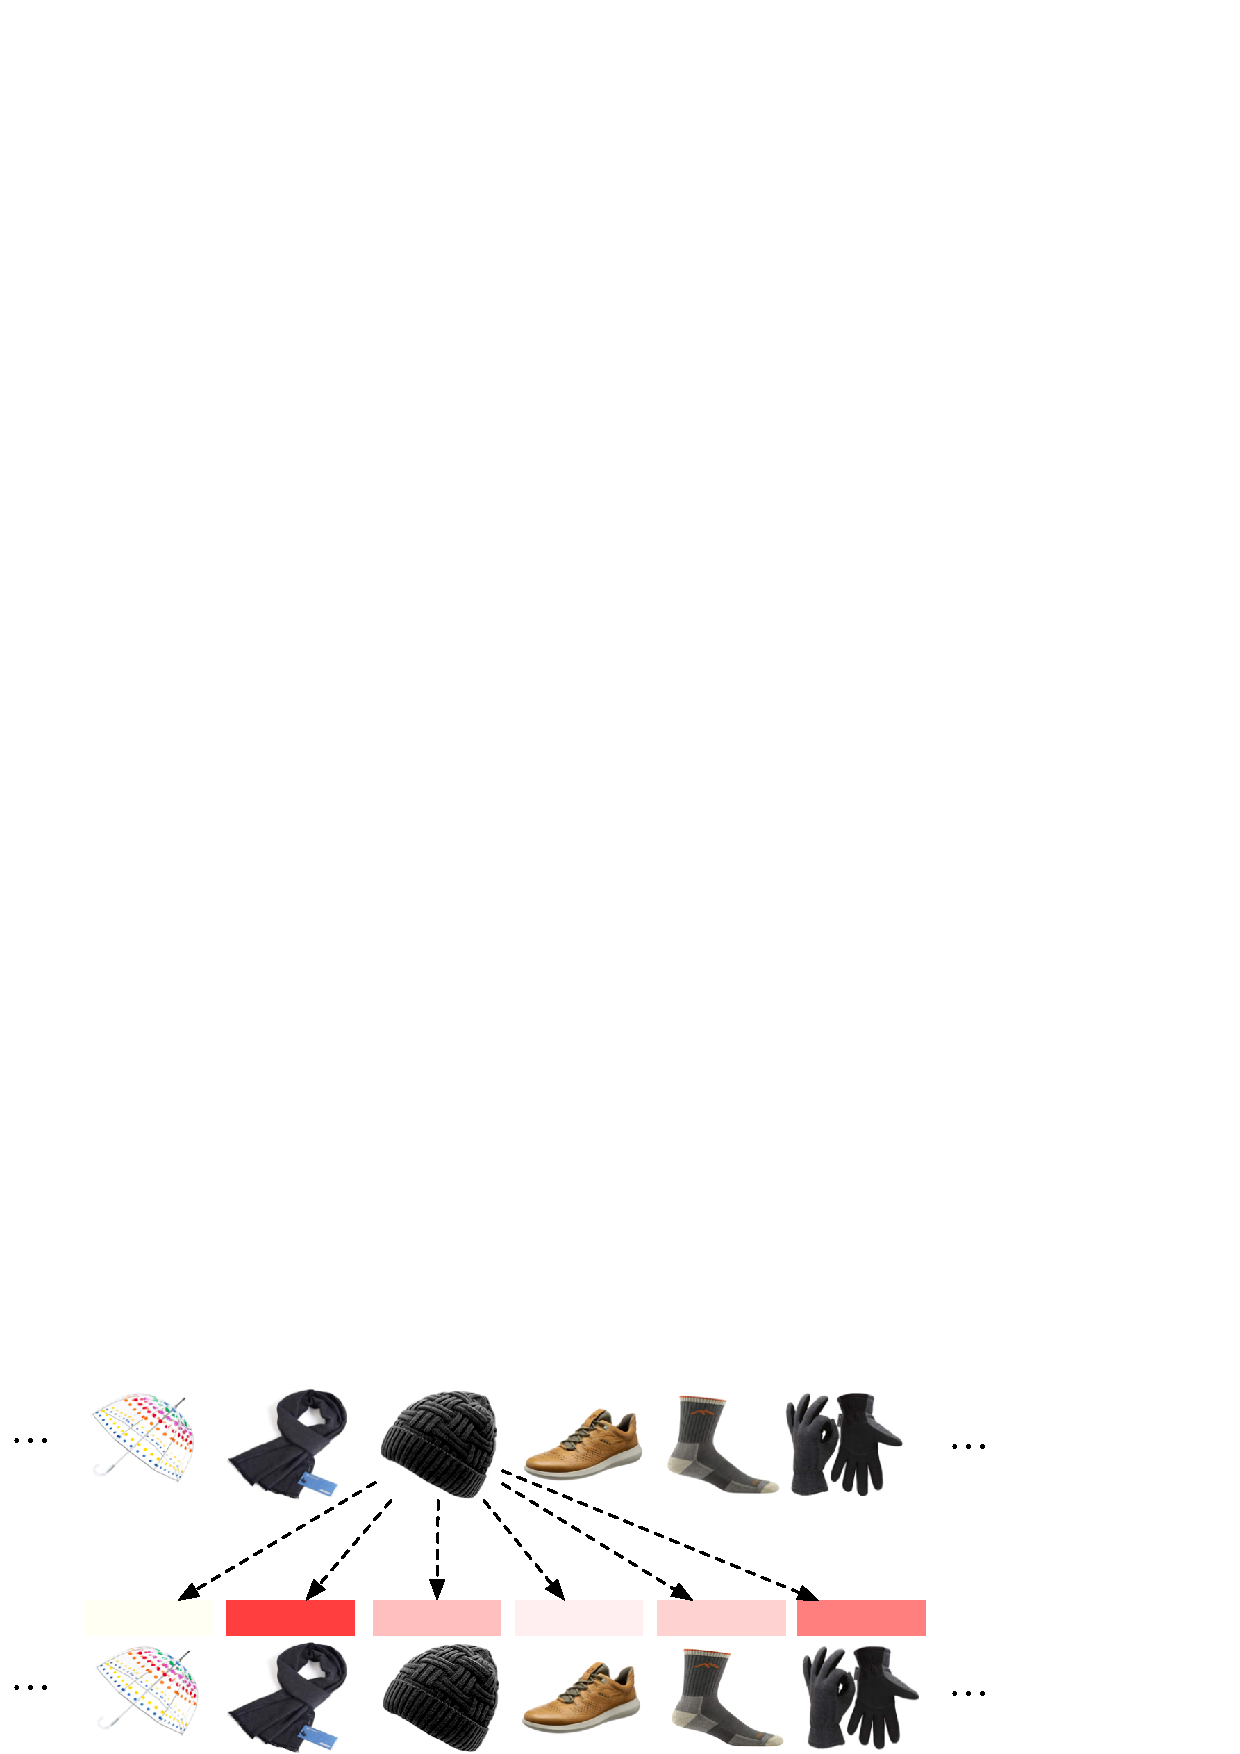
\includegraphics[width=1.0\columnwidth]{figure/attention.pdf}}
	\caption{Attention weight visualization. \textit{AtLocation} is required for prompt in the left column and \textit{PartOf} is required for prompt in the right column.} \label{fig:attention}
\end{figure}
Specifically, we focus on the attention weights between [MASK] token and 
other tokens in the prompt. A first glance of change of attention pattern 
is given in \figref{fig:LAMA} and we show more examples of other ConcetpNet 
relations in \figref{fig:attention}. We observe that while the original 
pretrained model tends to attend to special tokens like period and [SEP], 
the subnetwork successfully grasps the relevant concepts~(i.e., apple, 
worms, and basement) in the prompt hence produces the right object. 
We also use t-SNE~\citep{vanDerMaaten2008} to visualize the last layer's 
representation of [CLS] for each prompt. From \figref{fig:tsne}, the 
representations computed by original pretrained model are hardly separable as 
different types of knowledge are mixed together. In contrast, the pruned 
subnetwork can extract meaningful and disentangled representations for 
different commonsense relations.

\begin{figure}[th]
	\centering
	\scalebox{1.0}{\includegraphics[width=1.0\columnwidth]{figure/tsne_compare.pdf}}
	\caption{t-SNE visualization of [CLS]'s representation from original~(left) and pruned~(right) \textsc{BERT-base}.} \label{fig:tsne}
\end{figure}


\subsection{Commonsense Knowledge Base Completion~(CKBC)}
\label{sec:ckbc}
We evaluate the utility of identified relation-specific subnetworks on CKBC in an unsupervised manner. Specifically, we use the ConceptNet-100K benchmark provided by \citet{Li2016}. To ensure a fair evaluation, 
we manually create a subset of ConceptNet-100K 
consisting of triples with single-token subject/object. We also ensure that its dev/test set has \textbf{no overlap} with C-LAMA.
Each relation is associated with a sentence template~(provided in 
Appendix)~\citep{Kwon2019} of which the wording is distinct from 
those in C-LAMA. We acknowledge that these sentence templates might be suboptimal for certain relations, but prompt optimization is 
out of the scope of this paper. The resulting dataset contains 
$17,891$ training instances, $349$ development instances, 
and $446$ test instances.

\textbf{Link prediction.}~~We first formulate CKBC as a link prediction task 
and compare subnetworks~(i.e., $\mathcal{LM}_{\theta_r}$ 
is queried to predict missing link for instance of relation $r$) as well as original PLMs
against strong supervised KB completion mothods. 


\tabref{table:linkprediction} shows the results. Most of the supervised 
models outperform full-scale PLMs by a large margin, which suggests the 
inefficacy of directly using PLMs to perform link prediction. However, 
the subnetworks identified by our pruning procedure can
acquire performance on par with or better than state-of-the-art 
supervised models. Surprisingly, the pruned \textsc{DistilBERT} get the 
highest MRR, outperforming other larger and more advanced PLMs. 
\textsc{RoBERTa} struggles to predict correct objects, perhaps due to 
its larger vocabulary size compared to WordPiece~($50,265$ vs $30,522$) 
and less lexicon overlap~($53\%$ vs $59\%$) with the dataset.

%\KZ{It seems that our method (pruned models) don't work so well in the
%test set, compared to dev set. The scores for the same model between dev set and
%test set are also quite diff. Can you explain in this para?}

\textbf{Triple classification}~~We can also formulate CKBC as a triple classification task. Following ~\citet{Feldman2020}, we use estimated point-wise mutual information~(PMI) computed by pretrained language model as a surrogate of a triple's validity. An expectation-maximization-based Gaussian mixture clustering method is used and instances in the cluster with higher mean PMI are labeled as valid. 
\begin{table}[t]
	\centering
	\scriptsize
	\begin{tabular}{l|c}
		\toprule
		\textbf{Model} &  \textbf{F1 Score}\\
		\midrule
		\textsc{DistilBERT} & 74.1\\
		\textsc{DistilBERT}~(pruned) & \textbf{76.3}\\
		\midrule
		\textsc{BERT} & 73.7\\
		\textsc{BERT}~(pruned) & \textbf{76.7}\\
		\midrule
		\textsc{RoBERTa} &74.8 \\
		\textsc{RoBERTa}~(pruned) & \textbf{76.9}\\
		\midrule
		\textsc{MPNet} &76.5 \\
		\textsc{MPNet}~(pruned) & \textbf{78.0}\\
		\bottomrule
	\end{tabular}
	\caption{Triple classification on ConceptNet-100K.}
	\label{table:tripleclassification}
\end{table}
In our preliminary experiments, we found that the model pruned by the mask 
of a single relation might not be robust for PMI estimation and generally 
performed inferior to the intact model. 
In the same spirit as model ensembling, we then perform grid search over 
combinations of multiple knowledge, which is similar to what we did 
in zero-shot commonsense reasoning. For all four PLMs considered in 
\tabref{table:tripleclassification}, we observe that there exists one 
or multiple knowledge combinations delivering F1 score higher than the 
original models. 
%\KZ{Why is the difference between pruned and unpruned models
%not so big compared to link prediction?}

\textbf{Triple extraction.}~~We then investigate the ability of specialized 
subnetworks to extract novel commonsense knowledge triples absent 
from the dataset. We randomly sample 100 triples from the test set of 
ConceptNet-100K and for each sample use top-$K$ predictions from 
pruned \textsc{DistilBERT-base} as candidate objects. 
Three human annotators are asked to first determine the correctness of 
each candidate object and further determine their novelty~(i.e., not present 
in any of train/validation/test set) if deemed to be correct. 
The Fleiss Kappa inter-annotator agreement $\kappa$ is 0.66/0.65 
for precision and novelty, respectively.
\begin{figure}[t]
	\centering
	\scalebox{0.7}{\includegraphics[width=1.0\columnwidth]{figure/precision_novelty_2.pdf}}
	\caption{Precision-novelty curve with varied $K$.} \label{fig:extraction}
\end{figure}
\figref{fig:extraction} shows the change of precision-novelty with varied $K$. We observe a clear trade-off between the validity and novelty of triples extracted by the pruned model. As expected, a large $K$ inevitably makes noisy predictions but is more likely to extract unseen knowledge. For the purpose of knowledge enrichment, one might choose a large $K$ to ensure a desirable recall. We list the obtained novel triples in the Appendix D due to space limits.






\subsection{Commonsense Reasoning~(CSR)}
\label{sec:csr}
After identifying sparse subnetworks within PLMs that specialize in different commonsense knowledge, we now evaluate their generalization ability in the context of commonsense reasoning.
%One desirable outcome of our pruning procedure is the transformation from language representation to knowledge representation. We test if such subnetworks generalize in the context of commonsense reasoning.

\textbf{Many-shot learning.}~~We experiment with \textsc{BERT-base} and its deterministically pruned version using supervised fine-tuning on $7$ datasets: RTE~\citep{CambridgeJournals:6906264}, COPA~\citep{roemmele_choice_2011}, CommonsenseQA~\citep{talmor-etal-2019-commonsenseqa}, SWAG~\citep{zellers-etal-2018-swag}, HellaSWAG~\citep{DBLP:journals/corr/abs-1905-07830},   aNLI~\citep{DBLP:journals/corr/abs-1908-05739} and CosmosQA~\citep{huang-etal-2019-cosmos}. For each task, we identify the commonsense knowledge it might requires with a simple heuristic. Specifically, we obtain the five most frequent relations~(measured by how many times subject and object of certain relation appear in the context or answer) for each task and perform grid search over the combinations of these relationns. Then we take the union of masks for each relation and apply the resultant mask to the BERT as initialization for finetuning.
We repeat the training three times with different random seeds for each task. 
The  choice of mask combination for each task can be found in Appendix B.

The results in \tabref{table:finetuning} shows that, when initialized with proper weights, the model can be better fine-tuned on downstream commonsense reasoning tasks via more useful \textit{prior} knowledge. We further analyze the change of performance under the low-resource regime on COPA dataset. \figref{fig:copa} shows that the pruned \textsc{BERT} exhibits a notable advantage when training data is extremely scarce. As more training data is seen, the benefit of the pruned 
model becomes less prominent, i.e., $p>0.05$.
\begin{table}[t!]
	\centering
	\scriptsize
	\begin{tabular}{l|cc|c}
		\toprule
		\textbf{Task} & \textbf{Original} & \textbf{Pruned} &$p$-value \\
		\midrule
		RTE & 69.2$\pm${\scriptsize 2.3} & 69.8$\pm${\scriptsize2.0}& 0.12\\

		COPA & 62.4$\pm${\scriptsize 5.0} & 63.0$\pm${\scriptsize 4.7} &0.33  \\

		CommonsenseQA & 53.1$\pm${\scriptsize 0.6} & 54.1$\pm${\scriptsize 0.7} &0.08\\

		SWAG & 73.9$\pm${\scriptsize 0.3} & 74.2$\pm${\scriptsize 0.1} &0.09\\
		HellaSWAG & 38.9$\pm${\scriptsize 0.4} & 39.1$\pm${\scriptsize 0.5}&0.32  \\
		aNLI &63.7$\pm${\scriptsize 0.4} &64.0$\pm${\scriptsize 0.4}  &0.19\\
		CosmosQA &61.3$\pm${\scriptsize 1.0} &61.8$\pm${\scriptsize 0.2} &0.26\\
		\bottomrule
	\end{tabular}
	\caption{Finetuning results of \textsc{BERT} for CSR.}
	\label{table:finetuning}
\end{table}
\begin{figure}[t]
	\centering
	\scalebox{0.75}{\includegraphics[width=1.0\columnwidth]{figure/copa.pdf}}
	\caption{Finetuning result of \textsc{BERT} on COPA with varying portion of data.} \label{fig:copa}
\end{figure}
\begin{table*}[t!]
	\centering
	\scriptsize
	\begin{tabular}{l|cccccccc|c}
		\toprule
		\textbf{Model} &COPA-Tra. &COPA-Val. &CSQA &CA &WSC  &SM &ARCT1 &ARCT2 &Avg. \\
		\midrule
		\textsc{DistilBERT} &58.3 &60.0 &29.6 &84.6 &53.3  &71.6 &48.6 &50.4  &57.0  \\
		\textsc{DistilBERT}~(pruned) &\textbf{61.5} &\textbf{69.0} &\textbf{31.5} &\textbf{89.6} &\textbf{56.9}  &\textbf{72.1} &\textbf{53.4} &\textbf{51.6} & \textbf{60.7} \\
		\midrule
		\textsc{BERT} &60.2 &54.0 &26.5 &89.0 &57.3  &69.7 &46.8 &50.3 &56.7 \\
		\textsc{BERT}~(pruned) &\textbf{63.0} &\textbf{64.0} &\textbf{28.5} &\textbf{91.8} &\textbf{59.0}  &\textbf{71.7} &\textbf{50.0} &\textbf{52.0}  & \textbf{60.0}\\
		\midrule
		\textsc{RoBERTa} &60.7 &59.0 &39.9 &90.1 &61.8  &73.1 &48.6 &53.1 &60.7 \\
		\textsc{RoBERTa}~(pruned) &\textbf{65.3} &\textbf{72.0} &\textbf{40.4} &\textbf{93.4} &\textbf{62.9}  &\textbf{74.4} &\textbf{53.2} &\textbf{55.1} &\textbf{64.6}\\
		\midrule
		\textsc{MPNet} &66.5 &69.0 &40.0 &94.5 &64.3&75.8  &52.9 &56.7 &64.9  \\
		\textsc{MPNet}~(pruned) &\textbf{71.0} &\textbf{74.0} &\textbf{41.7} &\textbf{97.3} &\textbf{66.4}  &\textbf{77.5} &\textbf{56.1} &\textbf{57.7}  & \textbf{67.7}\\
		\bottomrule
	\end{tabular}
	\caption{Zero-shot results of accuracy~(\%) on commonsense reasoning tasks. Better results of each pair is in \textbf{bold}.}
	\label{table:zeroshot}
\end{table*}



\textbf{Zero-shot learning.}~~We next assess the ability of specialized 
subnetworks to perform zero-shot commonsense reasoning, a setting where 
the knowledge relied on to complete the task is solely determined by the model 
parameters. Here we focus on the following multiple-choice datasets: training set of COPA~(COPA-Tra.), validation set of COPA~(COPA-Val.), CommonsneseQA, Conjunction 
Acceptability~(CA)~\citep{Zhou2019}, 
Winograd Schema Challenge~(WSC)~\citep{levesque_winograd_2012}, 
SenseMaking~(SM)~\citep{wang-etal-2019-make}, 
ARCT1~\citep{habernal-etal-2018-argument} and 
ARCT2~\citep{DBLP:journals/corr/abs-1907-07355}. Each sample in the above datasets can be formulated as $\{[CLS]~context~[SEP]~choice_i ~[SEP]\}_{i=1}^{N}$, where $i$ is the subscript and $N$ is the number of choices. We compute the plausibility score of each choice using MLM head. Choice with the highest plausibility score is chosen as the answer. 

Since multiple types of knowledge are typically required for effectively 
reasoning over concepts, for each task, we perform grid search over 
combinations of $3$-$4$ different commonsense knowledge out of 
the $16$ total types and reported the best accuracy in \tabref{table:zeroshot}. 
We put the best combination for each model on each task in Appendix B
for space constraints. By combining multiple commonsense knowledge useful for the task, 
we show that the pruned models can actually surpass their full-scale 
version in all tasks considered in our experiments. 
The most likely explanation is that knowledge irrelevant to the specific task 
in the original models hurt the in-domain zero-shot reasoning capability. 
It also manifests that the most important reasoning skills vary from 
task to task.


\section{Related Work}
This section surveys previous works on question generation and tree encoding
respectively.

Text question generation has attracted the attention 
after the work of ~\citeauthor{du2017learning}~\shortcite{du2017learning}, who uses deep seq2seq model 
to generate questions from a raw text paragraph. 
Before that, text question generation relied heavily on hand-craft 
question patterns~\cite{HeilmanS10,LabutovBV15,MostowC09} which is time and 
labor consuming. 

However, this pure seq2seq model is not focused and 
has no control over part in the paragraph to generate question. 
~\citeauthor{zhou2017neural}~\shortcite{zhou2017neural} proposed to encode 
key phrase information using binary indicators to generate 
key-aware questions and they assumes the answer to be key phrase. 
Considering key phrase (answer) is unavailable in reality, 
~\citeauthor{SubramanianWYT17}~\shortcite{SubramanianWYT17} applied 
a two-stage approach. First, key phrases are extracted by 
pointer network~\cite{ptrnet}. Second, 
key phrases are encoded in the same way as 
Zhou et al. With the intuition that questions could be asked in many ways, 
~\citeauthor{Yao2018vae}~\shortcite{Yao2018vae} used conditional-VAE to 
increase the diversity of questions. More recently, models with 
auxiliary feature information~\cite{HarrisonW18} helped improve 
the question quality. Structure question generation aims at 
converting structured data such as triples in knowledge graph to questions. 
~\citeauthor{SerbanGGACCB16}~\shortcite{SerbanGGACCB16} proposed a model to generate factoid questions from knowledge base triples.  None of the above work
considered using parse tree structures to aid question generation process,
which is the focus of this paper.

Sequential RNN model takes sentence as a sequence of words, 
ignoring the syntactic information. In order to utilize
such syntactic information with sequential information, 
~\citeauthor{tai2015improved}~\shortcite{tai2015improved} proposed Tree-LSTM to 
encode the binary parse tree recursively in a bottom-up fashion to 
classify sentiment. In text generation task, 
\citeauthor{eriguchi2016tree}~\shortcite{eriguchi2016tree} 
proposed a tree-to-sequence model with attention mechanism to do 
machine translation and 
~\citeauthor{liang2018automatic}~\shortcite{liang2018automatic} proposed a 
tree-to-sequence model which could handle arbitrary trees, 
to do code comment generation. Our work is inspired by these previous
attempts and we are first to adapt structure encoded neural models to
textual question generations.

\section{Conclusion}
\label{sec:conclude}
Ad hoc data sources
are extremely difficult to manage because of their large size,
evolving format, and lack of documentation.
In this paper, we have presented the design, implementation and
evaluation of a system for incrementally learning the structure of 
large or stream ad hoc data files. The output of the
system is a data description in \pads{} language which can further
generate end-to-end data processing tools. 
The system allows the users to get into the iterative learning process
and make the description more accurate and readable.

%\paragraph*{Acknowledgements.}
%This work was partially supported by NSFC Grants No. 61033002 and 61100050
%and by NSF grant CCF-1016937. Any opinions, findings, and recommendations
%expressed in this material are those of the authors and do not
%necessarily reflect the views of these agencies.
%The system not only
%produces documentation for the files in the form of a \pads{}
%description, but it can also be used to generate end-to-end
%data processing tools such as a statistical analysis or an
%XML translator.  
%We have shown that the system
%can scale to the point where it can process and learn the
%structure of logs on the order of up to 30GB or more in 
%a few hours.

{\renewcommand{\baselinestretch}{0.9}
\small
\bibliographystyle{plain}
\bibliography{pads}
}

\end{document}


